\section{MisUse Cases}

Use Cases spielen nicht nur bei der Softwareentwicklng eine bedeutende Rolle beim requirements engineering. Es ist jedoch in der UML 2 Spezifikation nicht möglich Sicherheitsanalysen mit Use Cases durchzuführen \cite{sindre2005eliciting}. 
In \cite{sindre2005eliciting} wird eine Erweiterung von Use Cases vorgestellt, die es auch ermöglicht Missbrauch darzustellen. Während Use Cases etwas von Wert für den Systembesitzer und Stakeholder schaffen, stellen Misuse Cases einen Schaden am System und Werten dar.
Misuse Case und Misuser werden dabei wie folgt definiert.
\begin{quote}
\textbf{Misuse Case} A sequence of actions, including variants, that a system or other entity can perform, interacting with misusers of the entity and causing harm to some stakeholder if the sequence is allowed to complete. \cite{sindre2005eliciting}
\end{quote}

\begin{quote}
\textbf{Misuser} An actor that initiates misuse cases, either intentionally or inadvertently. \cite{sindre2005eliciting}
\end{quote}

Wie bei normalen Use Cases werden die Relationen \textit{include}, \textit{association}, \textit{extend} und \textit{generalize} verwendet.
In \cite{sindre2005eliciting} werden folgende neue Relationen beschrieben:
\begin{itemize}
\item \textit{mitigate/prevent} Der Use Case ist eine Gegenmaßnahme gegen einen Misuse Case. Er reduziert also die Erfolgswahrscheinlichkeit.
\item \textit{threaten} Ein Misuse Case kann einen Use Case gefährden und bei der Ausführung hindern.
\end{itemize}

Seamonster sieht außerdem Vulnerabilities, also Schwachstellen vor, die im Diagramm als graue Use Cases dargestellt werden. Diese Schwachstellen werden von einem Insider verursacht und können von einem Misuse Case mit der \textit{exploit} Relation ausgenutzt werden.

\subsection{Textuelle Spezifikation}
Misuse Cases lassen sich ähnlich regulärer Use Cases darstellen. Tabelle~\ref{tab:MisuseCaseTemplate} zeigt das hierfür verwendete Template. 

\begin{table}
\scriptsize
\centering
\caption{Template für eine ausführliche Misuse Case darstellung aus \cite{sindre2005eliciting}}
\label{tab:MisuseCaseTemplate}
\begin{tabular}{p{0.2\textwidth}p{0.8\textwidth}}
\hline 
Name, Summary, Author,
and Date: & These fields retain the same meaning as in regular use cases \\ 
\hline 
Basic path: & This field describes the actions that the misuser(s) and the system go through to harm the
proposed system \\ 
\hline 
Alternative paths: & This field describes ways to harm the proposed system that are not accounted for by the basic path,
but are still sufficiently similar to be described as variants of the basic path \\ 
\hline 
Mitigation points: & This field identifies those actions in a basic or alternative path where misuse can be mitigated.
Several ways to mitigate misuse of a particular action can be described in the same field and
each of them may be further described in a separate security use case. As for extension
points, the misuse case must eventually have a mitigate relationship to a corresponding
security use case. However, the detailed description of security use cases is optional, because
it is often closer to design, requiring detailed analysis of risks and implementation
costs that go beyond use and misuse cases \\ 
\hline 
Extension points: & In some cases, a misuse case may be extended with optional paths whose details are described
in a separate extension misuse case. This field lists the actions in the main or alternative paths
where optional paths may be inserted. As for extension points in regular use cases, the misuse
case must have an extend relationship to the misuse case that contains the optional path \\ 
\hline 
Trigger: & This field describes the states or events in the system or its environment that may initiate the
misuse case. For some misuse cases, the trigger is just the predicate True, indicating
a permanently present danger \\ 
\hline 
Assumptions: & This field describes the states in the system’s environment that make the misuse case possible \\ 
\hline 
Preconditions: & This field describes the system states that make the misuse case possible \\ 
\hline 
Mitigation guarantee: & This field describes the guaranteed outcome of mitigating a misuse case. If the mitigation points
are not yet specified in detail, the mitigation guarantee describes the level of security required
from the mitigating security use cases that will be designed later. When the mitigation points
in the misuse case have been detailed by security use cases, this field describes the strongest
possible security guarantee that can be made, regardless of how the misuse case is mitigated \\ 
\hline 
Related business rules: & Typically, business rules will be violated by the misuse. This field contains links to
such rules, maybe along with links to rules that enable the threat or that limit
how it could be mitigated or eliminated \\ 
\hline 
Misuser profile: & This field describes whatever can be assumed about the misuser, for example, whether the misuser
acts intentionally or inadvertently; whether the misuser is an insider or outsider; and how
technically skilled the misuser must be \\ 
\hline 
Scope: & This field indicates whether the proposed system in a misuse case is, e.g., an entire business,
a system of both users and computers, or just a software system \\ 
\hline 
Iteration: & As for regular use cases, it is useful to allow both initial and detailed descriptions of misuse
cases. This field indicates the misuse case’s iteration level, usually taken from the set of
iteration levels used for the use cases in the project \\ 
\hline 
Level: & As for regular use cases, misuse cases can be specified at a general or specific
abstraction level. This field indicates whether the misuse case is, e.g., a summary,
a user goal, or a sub-function, following \\ 
\hline 
Stakeholders and risks: & This field specifies the major risks for each stakeholder involved in the misuse case. On an abstract
level, risks can be described textually, e.g., ‘‘the system is unavailable for several hours’’ or
‘‘a competitor gets hold of sensitive medical data about an applicant’’. On a concrete level,
the likelihood and cost of each misuse variant can be estimated, where the cost includes potential
losses, should the threats come true \\ 
\hline 
Technology and data variations: & A misuser may carry out a misuse case from a variety of technical platforms, such as a PC
or a WAP phone and, since only a few equipment-related actions will differ in each case,
it is unnecessary to specify two separate paths. Instead, this field lists the candidate types
of equipment and explains how they differ in particular actions \\ 
\hline 
Terminology and explanations: & This field contains explanations of technical terms and other issues \\ 
\hline 
\end{tabular} 
\end{table}

\subsection{Misuse Case Diagramme}
Wie Use Case Diagramme, dienen Misuse Case Diagramme der Übersicht und verbindung mehrerer Use Cases bzw. Misuse Cases. Fowler beschreibt das Use Case Diagramm in \cite{fowler2004uml} als nützlich aber nicht notwendig und empfiehlt sich auf die textuelle Darstellung zu konzentrieren. 

Seamonster unterstützt nur die Darstellung der Diagramme, nicht aber die textuelle Darstellung.

\subsection{Anwendung auf die Fallbeispiele}
Die folgenden Misuse Cases und Misuse Case Diagramme geben einen Überblick über die Sicherheitsanforderungen für beide Fallbeispiele. Da sich im Bereich der Misuse Cases für beide Fallbeispiele wenig Unterschiede ergeben haben, wird nicht zwischen FB I \& II differenziert.

\subsubsection{Diagramme}

\begin{figure}[h]
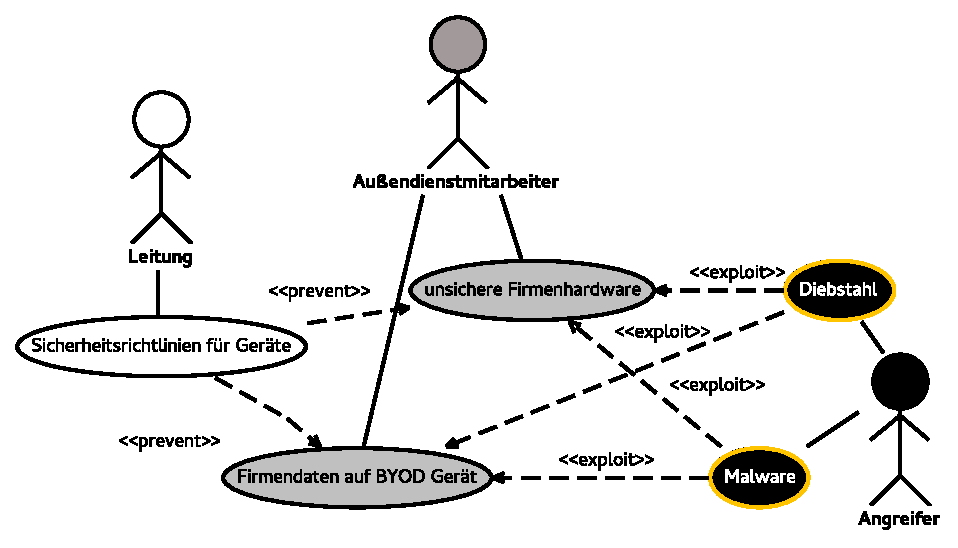
\includegraphics[scale=0.8]{images/Hardware.pdf} 
\caption{Misuse Case Diagramm für den Missbrauch von Außendienstmitarbeiterhardware. Sicherheitsrichtlinien für Geräte (z.B. Verschlüsselung) können Angriffe erschweren oder verhindern.}
\end{figure}

\begin{figure}[h]
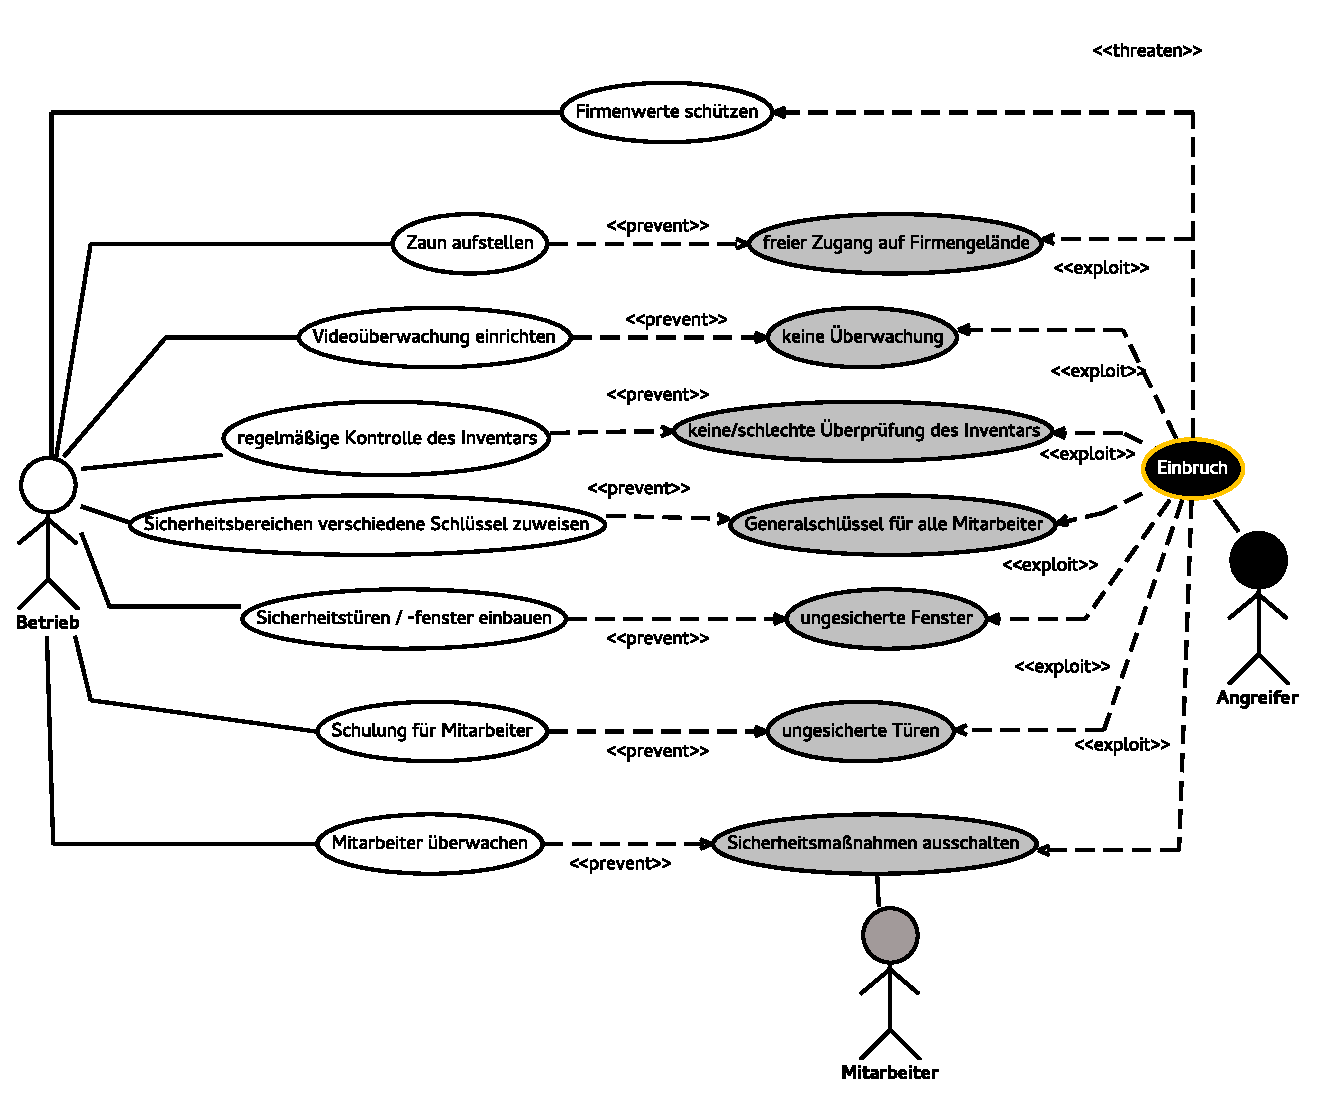
\includegraphics[scale=0.8,angle=90]{images/MisUseCaseEinbruch.pdf} 
\caption{Misuse Case Diagramm für ein Einbruchsszenario. Dem Angreifer werden verschiedene Sicherheitsmaßnahmen entgegengestellt, die einen Einbruch verhindern oder erschweren können}
\end{figure}


\begin{figure}[h]
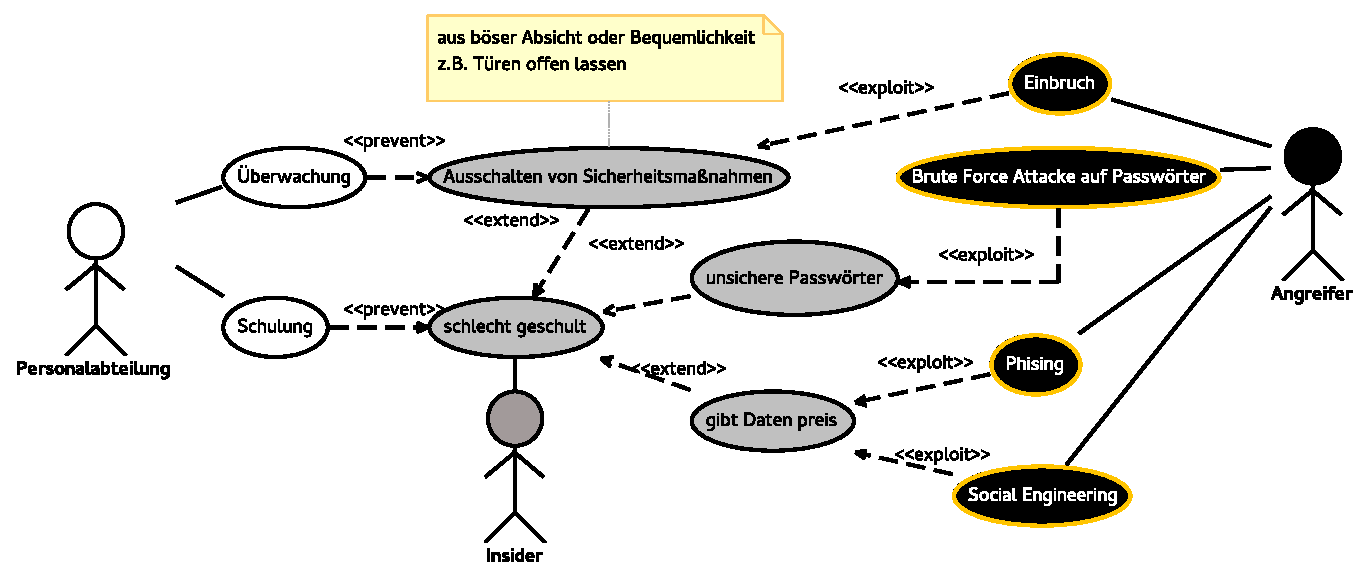
\includegraphics[scale=0.8,angle=90]{images/Schulung.pdf} 
\caption{Misuse Case Diagramm welches die Vorteile von Mitarbeiter Schulungen aufzeigt.}
\end{figure}

\begin{figure}[h]
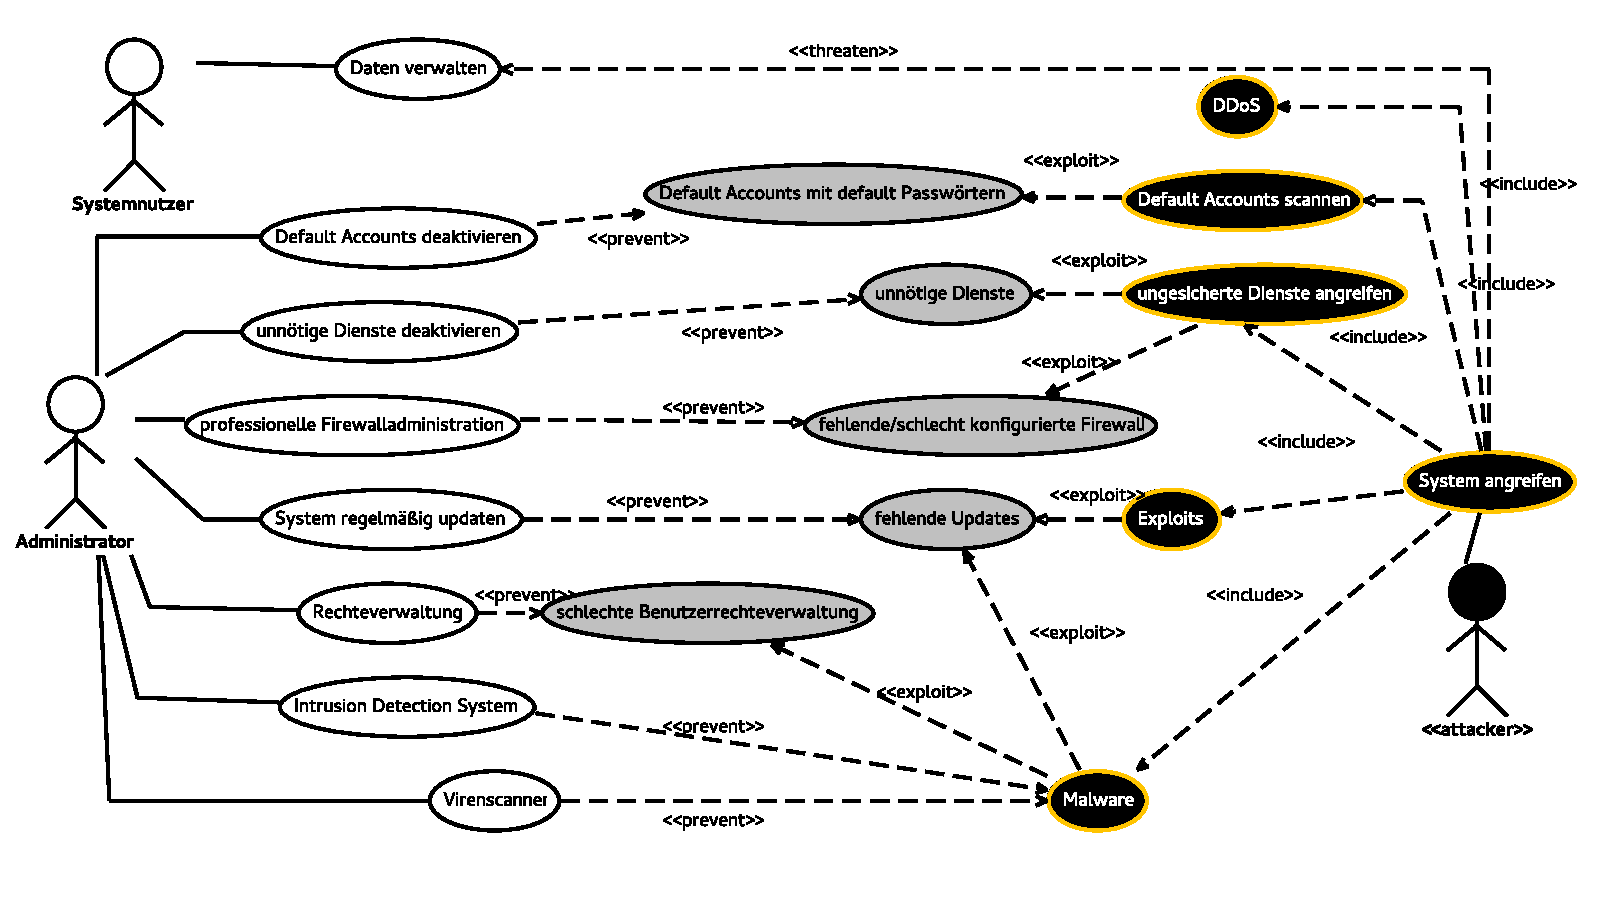
\includegraphics[scale=0.8,angle=90]{images/Server.pdf} 
\caption{Misuse Case Diagramm für mögliche Angriffsszenarien auf Serversysteme. Dabei werden nur Angriffe über das Netzwerk berücksichtigt und physischer Zugriff nach einem Einbruch außen vor gelassen.}
\end{figure}

\clearpage
\subsubsection{Textuelle Darstellung}

\begin{table}[h]
\scriptsize
\centering
\caption{Misuse Case: Missbrauch von Außendienstmitarbeiterhardware}
\label{tab:MisuseCaseTemplate}
\begin{tabular}{p{0.2\textwidth}p{0.8\textwidth}}
\hline 
Name: & Missbrauch von Außendienstmitarbeiterhardware \\ 
\hline 
Summary: & Ein Angreifer versucht über die Hardware von Außendienstmitarbeitern Zugang auf Firmendaten zu erlangen.\\
\hline
Basic path: & bp-1. Der Angreifer versucht Malware auf die ungesicherte Hardware zu schleusen. Dazu nutzt er ein ungesichertes und unbeaufsichtigtes Gerät.\\
 & bp-2. Der angreifer stielt ein ungesichertes und unbeaufsichtigtes Gerät um später Zugriff auf die Daten zu erhalten.\\ 
\hline 
Mitigation points: & mp1. Sicherheitsrichtlinen für Geräte, wie z.B. Verschlüsselung, Automatische Sperrung bei Inaktivität, Virenschutz, Verbot von eigenen Geräten, etc. können den Angriff erschweren oder unmöglich machen. Sollte der ANgreifer nur die Hardware stehlen wollen und nichts mit den Firmendaten anfangen können,so bleibt der Verlust relativ gering, solange Backups existieren.\\ 
\hline 
Trigger: & Der Außendienstmitarbeiter lässt seinen Laptop oder ein anderes Gerät mit Firmendaten für kurze Zeit unbeaufsichtigt. Dies erleichtert den Angriff nur. Ein Diebstahl ist immer möglich.\\ 
\hline 
Preconditions: & Der Außendienstmitarbeiter speichert Firmendaten auf unsicherer Hardware.\\ 
\hline 
Mitigation guarantee: & Der Angreifer kann keine Malware einschleusen, da der Rechner gesperrt und/oder passwortgesichert ist (bp-1). Der Angreifer kann mit gestohlener Hardware nichts anfangen, da alle Daten verschlüsselt sind (bp-2).\\ 
\hline 
Misuser profile: & Der Angreifer ist ein Mitarbeiter der Konkurrenz, Industriespion oder jemand, der nur die Hardware möchte. \\ 
\hline 
Scope: & Kompletter Betrieb \\ 
\hline 
Stakeholders and risks: & Sollten wichtige Forschungs- oder Produktionsdaten gestohlen und an die Konkurrenz verkauft werden, so können schwere Verluste für das Unternehmen entstehen. \\ 
\hline 
\end{tabular} 
\end{table}